\documentclass[a4paper,11pt]{report}
\usepackage[top=2cm, bottom=2cm, left=2.5cm, right=2.5cm]{geometry}
\usepackage[utf8]{inputenc}
\usepackage{cmap}
\usepackage{graphicx} 
\usepackage[T2A]{fontenc}
\usepackage[english,russian]{babel}
\usepackage{amsmath}
\usepackage{amsfonts}
\usepackage{listings}
\usepackage{multirow}
\usepackage{hhline}
\usepackage{float}

% Title Page
\title{Отчёт по практическому заданию №1 ``Прямые и итерационные методы решения СЛАУ''}
\author{Маслов Н.С. группа 205}

\lstset{
language=C,
breaklines=true,
basicstyle=\small\ttfamily,
numbers=left,
numberstyle=\tiny,
frame=tb,
columns=fullflexible,
showstringspaces=false,
extendedchars=\true,
keepspaces=true
}

\floatstyle{ruled}
\newfloat{bash}{H}{lop}
\floatname{bash}{Консоль}

\begin{document}
\begin{titlepage}

\newgeometry{top=2.5cm, left=2.5cm, right=2.5cm}



\center % Center everything on the page
 
%----------------------------------------------------------------------------------------
%	HEADING SECTIONS
%----------------------------------------------------------------------------------------

\textsc{\Large Московский государственный университет им. М.В.Ломоносова}\\[0.5cm] % Name of your university/college
\textsc{\Large Факультет вычислительной математики и кибернетики}\\[7.5cm] % Major heading such as course name

%----------------------------------------------------------------------------------------
%	TITLE SECTION
%----------------------------------------------------------------------------------------

\textsc{\LARGE Отчёт о выполнении практической работы № 2}\\[1cm]
\textsc{\LARGE \huge \bfseries Численные методы решения дифференциальных уравнений}\\[5cm] % Title of your document
 
%----------------------------------------------------------------------------------------
%	AUTHOR SECTION
%----------------------------------------------------------------------------------------

\begin{minipage}{0.4\textwidth}
\begin{flushleft} \large

\end{flushleft}
\end{minipage}
~
\begin{minipage}{0.4\textwidth}
\begin{flushright} \large
Выполнил \\[0.3cm]
Маслов Н.C. \\ группа 205 % Your name
\end{flushright}
\end{minipage}\\[4cm]

% If you don't want a supervisor, uncomment the two lines below and remove the section above
%\Large \emph{Author:}\\
%John \textsc{Smith}\\[3cm] % Your name

%----------------------------------------------------------------------------------------
%	DATE SECTION
%----------------------------------------------------------------------------------------

{\large Москва, 2014}\\[3cm] % Date, change the \today to a set date if you want to be precise

%----------------------------------------------------------------------------------------
%	LOGO SECTION
%----------------------------------------------------------------------------------------

%\includegraphics{Logo}\\[1cm] % Include a department/university logo - this will require the graphicx package
 
%----------------------------------------------------------------------------------------

\vfill % Fill the rest of the page with whitespace

\end{titlepage}

%\tableofcontents

\section*{Подвариант №1. Решение задачи Коши для дифференциального уравнения первого порядка или системы дифференциальных
уравнений первого порядка}

\subsection*{Постановка задачи}

Рассматривается обыкновенное дифференциальное уравнение первого порядка, разрешённое относительно производной и имеющее вид:

$$ 
\frac{dy}{dx} = f(x, y), x_0 < x,
$$

с дополнительным начальным условием, заданным в точке $x = x_0$:

$$
y(x_0) = y_0.
$$

Предполагается, что правая часть уравнения - функция $f = f(x, y)$ такова, что гарантирует существование и единственность решения
задачи Коши.

В том случае, если рассматривается не одно дифференциальное уравнение, а система ОДУ первого порядка, разрешённых относительно
производных неизвестных функций, то соответствующая задача Коши имеет следующий вид:

$$
\begin{cases}
 \frac{dy_1}{dx} = f_1(x, y_1, y_2), \\
 \frac{dy_2}{dx} = f_2(x, y_1, y_2), x_0 < x
\end{cases}
$$

Дополнительные (начальные) условия задаются в точке $x = x_0$:

$$
y_1(x_0) = y_1^{(0)}, y_2(x_0) = y_2^{(0)}
$$

Также предполагается, что правые части уравнений заданы так, что это гарантирует существование и единственность решения задачи Коши, но
уже для системы обыкновенных дифференциальных уравнений первого порядка в форме, разрешённой относительно производных неизвестных 
функций.

\subsection*{Метод решения}

Для решения применяем метод Рунге-Кутта решения разностного уравнения.

Рассмотрим правую часть разностного уравнения:

$$
\frac{y_{i+1} - y_i}{h} = f(x_i, y_i) + \frac{1}{2}\Big\{\frac{\partial f}{\partial x}(x_i, y_i) + \frac{\partial f}{\partial y}
(x_i, y_i)f(x_i, y_i)\Big\}h
$$

Главная идея метода Рунге-Кутта состоит в том, чтобы приближённо заменить её на сумму значений функции $f$ в двух разных точках с 
точностью до членов порядка $h^2$. Если положить

$$
f(x_i, y_i) + \frac{1}{2}\Big\{\frac{\partial f}{\partial x}(x_i, y_i) + \frac{\partial f}{\partial y}
(x_i, y_i)f(x_i, y_i)\Big\}h = \beta f(x_i, y_i) + \alpha f(x_i + \gamma h, y_i + \delta h) + o(h^2),
$$

где $\alpha, \beta, \gamma, \delta$ - свободные параметры, которые необходимо подобрать; разложить функцию $f(x_i + \gamma h, y_i + \delta h)$
по степеням $h$ и таким образом выразить параметры $\beta, \gamma, \delta$ через $\alpha$, то получим уравнение для \textbf{однопараметрического
семейства разностных схем Рунге-Кутта}:

$$
\frac{y_{i+1} - y_i}{h} = (1 - \alpha)f(x_i, y_i) + \alpha f\Big(x_i + \frac{h}{2\alpha}, y_i + \frac{h}{2\alpha}f(x_i, y_i)\Big).
$$

В частности, наиболее удобные разностные схемы получаются при значениях параметра $\alpha$: $\alpha = 1/2$ и $\alpha = 1$. При решении
задач будем использовать значение $\alpha = 1/2$, задающее схему вычислений ``предиктор - корректор''.

Для решения систем дифференциальных уравнений первого порядка вычисления незначительно усложняются (для метода Рунге-Кутта второго порядка):

$$
y_{1,i+1} = y_{1, i} + \frac{1}{2} \Big(f_1(x_i, y_{1, i}, y_{2, i}) + f_1(x_i, \tilde{y}_{1, i}, y_{2, i})\Big),
$$
$$
y_{2,i+1} = y_{2, i} + \frac{1}{2} \Big(f_2(x_i, y_{1, i}, y_{2, i}) + f_2(x_i, y_{1, i}, \tilde{y}_{2, i})\Big),
$$
$$
\tilde{y}_{k, i} = y_{k, i} + f_k(x_i, y_{k, i}, y_{k, i})h, k = 1, 2.
$$

\subsection*{Описание программы}

Программа после сборки запускает выбранный аргументом командной строки тест, на стандартный поток вывода при этом выводится
таблица значений функций.

  ./diffeq test\_num

В первой колонке вывода записываются значения x. В следующих $2n$ колонках ($n = 1, 2$) выводятся значения полученных в результате вычисления
сеточных функций $y_1(x), ..., y_n(x)$ последовательно со значениями аналитически полученными решениями. 

В последней строке выводится значение получившейся ошибки вычисления, выбранной как максимум модуля расхождения аналитического и 
численного решения.

Программа реализует вычисление численного решения дифференциального уравнения методом Рунге-Кутта второго и четвёртого порядков
точности, а также вычисление численного решения системы двух дифференциальных уравнений методом Рунге-Кутта второго порядка.

\subsection*{Тесты}
В качестве результатов тестирования предлагаются графики функций (одновременно построенные для полученного решения и заранее 
вычисленного аналитического решения).

Во всех тестах взят отрезок $[0,2]$, шаг сетки 0.01.

\subsubsection{Тест 1}
Номера тестов в программе 1, 2.

Дано дифференциальное уравнение первого порядка и начальные условия

$$
y' = 3 - y - x, \\
y(0) = 0
$$

Аналитическое решение задачи Коши:

$$
y = 4 - x - e^{-x}
$$

Результат работы метода Рунге-Кутта второго порядка точности, 
максимальная ошибка составила $6.15438 \cdot 10^{-6}$


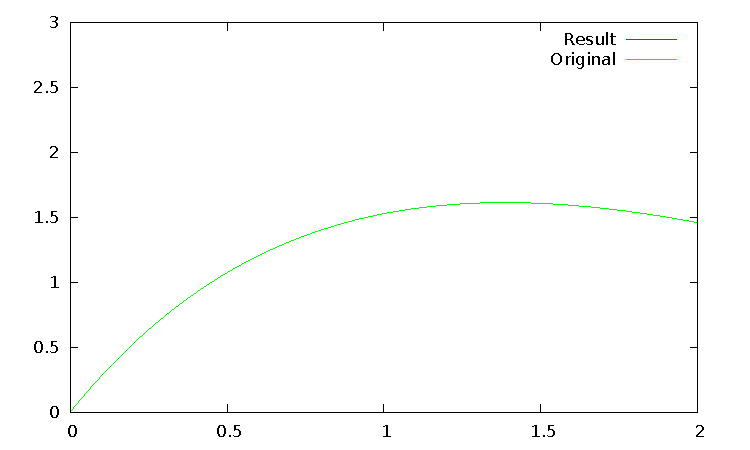
\includegraphics{../plots/test1_rk2.pdf}

Из значения максимальной ошибки вычисления ясно, что на этом уравнении метод должен дать очень
близкое решение.

Для метода Рунге-Кутта четвёртого порядка точности графики также практически совпадают, максимальная
ошибка составила $7.69496 \cdot 10^{-12}$.

\subsubsection{Тест 2 (предложенный вариант)}
Номера тестов в программе 3, 4.

Дано дифференциальное уравнение первого порядка с начальными условиями
$$
y' = \sin x - y, \\
y(0) = 10
$$

Предложенное аналитическое решение задачи Коши:
$$
y = -0.5 \cos x + 0.5 \sin x + \frac{21}{2}e^{-x}
$$

Результат работы метода Рунге-Кутта второго порядка точности, максимальная ошибка $1.59266 \cdot 10^{-5}$

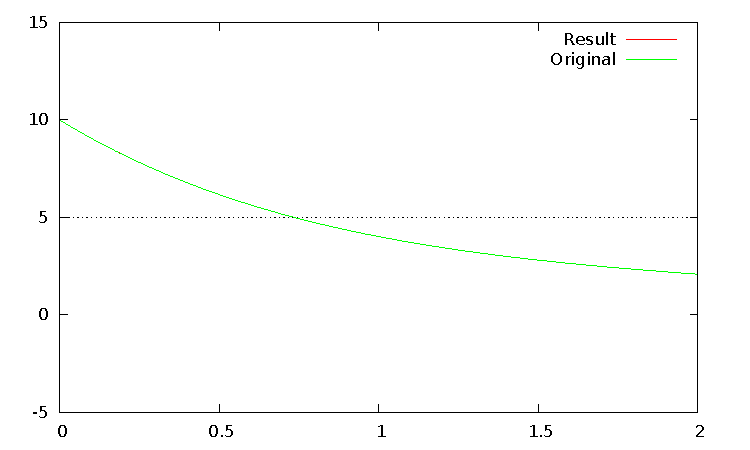
\includegraphics{../plots/test2_rk2.pdf}

Из значения максимальной ошибки вычисления ясно, что на этом уравнении метод должен дать очень
близкое решение.

Для метода Рунге-Кутта четвёртого порядка точности графики также практически совпадают, максимальная
ошибка составила $1.99263 \cdot 10^{-11}$.

\subsubsection{Тест 3}
Номера тестов в программе 5, 6.

Дано дифференциальное уравнение первого порядка с начальными условиями
$$
y' = -y - x^2, \\
y(0) = 10
$$

Предложенное аналитическое решение задачи Коши:
$$
y = -x^2 + 2x - 2 + 12 e ^ {-x}
$$

Результат работы метода Рунге-Кутта второго порядка точности, максимальная ошибка $1.11684 \cdot 10^{-5}$

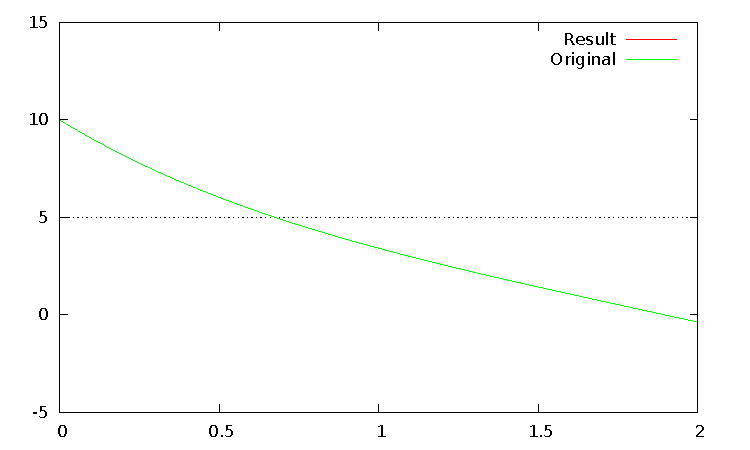
\includegraphics{../plots/test3_rk2.pdf}

Из значения максимальной ошибки вычисления ясно, что на этом уравнении метод должен дать очень
близкое решение.

Для метода Рунге-Кутта четвёртого порядка точности графики также практически совпадают, максимальная
ошибка составила $1.53788 \cdot 10^{-11}$.

\subsubsection{Тест 4, система уравнений}
Номер теста в программе: 7.

Дана система дифференциальных уравнений первого порядка с начальными условиями
$$
\begin{cases}
 x' = x + y, \\
 y' = x + y
\end{cases},
x(0) = 3, y(0) = 1
$$

Аналитическое решение системы
$$
\begin{cases}
 x = 1 + 2 e^{2t}, \\
 y = -1 + 2 e^{2t}
\end{cases}
$$

Результат работы метода Рунге-Кутта второго порядка точности для решения системы дифференциальных уравнений, максимальная
ошибка составила $1.08293$ (это связано с тем, что функции-решения достаточно быстро растут)

График функции x(t):

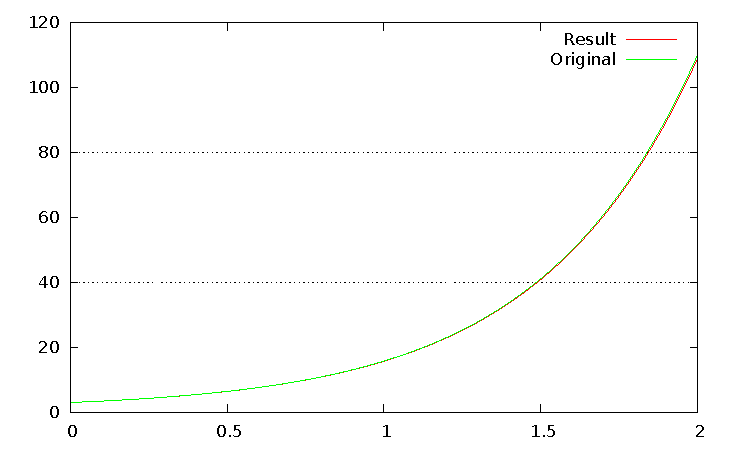
\includegraphics{../plots/test4_1.pdf}

График функции y(t):

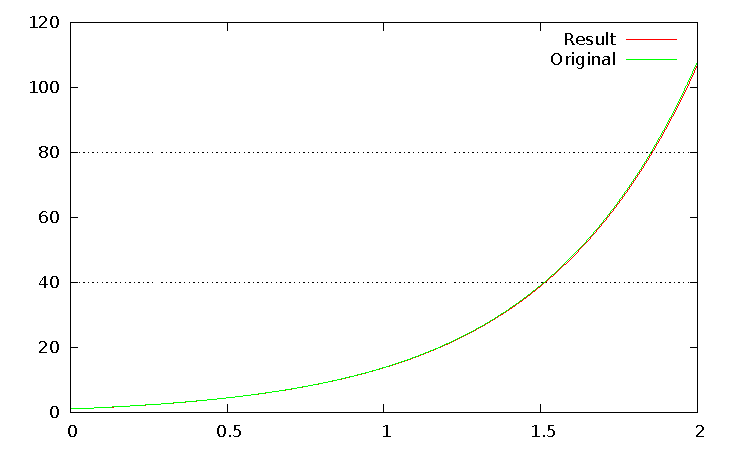
\includegraphics{../plots/test4_2.pdf}

\subsubsection{Тест 5, система уравнений (предложенный вариант)}
Номер теста в программе: 8.

Дана система дифференциальных уравнений первого порядка с начальными условиями
$$
\begin{cases}
 x' = \cos (t + 1.1y) + x, \\
 y' = -y^2 + 2.1x + 1.1
\end{cases},
x(0) = 0.25, y(0) = 1
$$

Аналитическое решение системы получить не удалось.

Результат работы метода Рунге-Кутта второго порядка точности для решения системы дифференциальных уравнений:

График функции x(t):

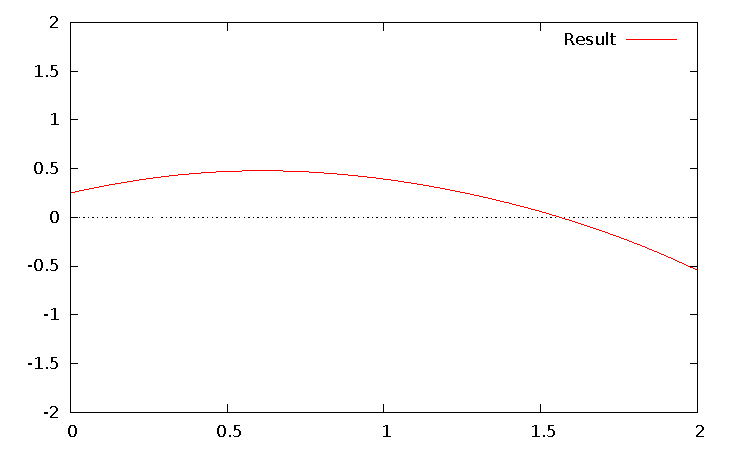
\includegraphics{../plots/test5_1.pdf}

График функции y(t):

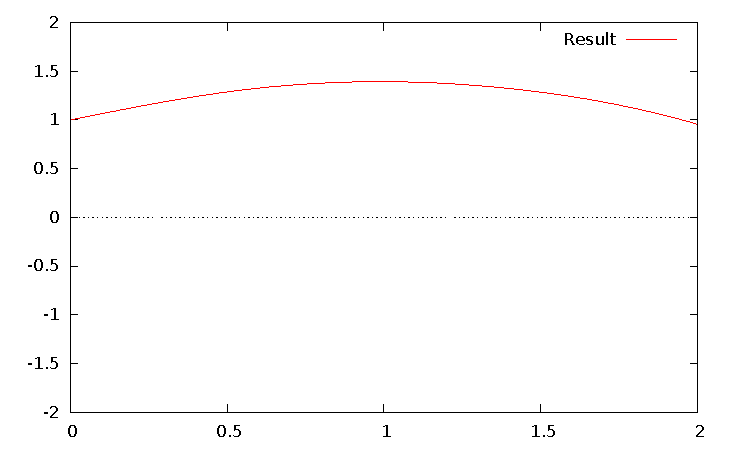
\includegraphics{../plots/test5_2.pdf}

\subsection*{Исходный код}

\lstinputlisting[caption={Решение дифференциального уравнения (системы ДУ) методом Рунге-Кутта (файл runge-kutta.c)}]{../runge-kutta.c}
\lstinputlisting[caption={runge-kutta.h}]{../include/runge-kutta.h}

\newpage

\section*{Подвариант 2. Решение краевой задачи для обыкновенного дифференциального уравнения второго порядка, разрешённого
относительно старшей производной}

\subsection*{Постановка задачи}

Рассматривается линейное дифференциальное уравнение второго порядка вида

$$
y'' + p(x) \cdot y' + q(x) \cdot y = - f(x), 1 < x < 0
$$

с дополнительными условиями в граничных точках 
$$
\begin{cases}
 \sigma_1 y(0) + \gamma_1y'(0) = \delta_1,\\
 \sigma_2 y(1) + \gamma_2y'(1) = \delta_2
\end{cases}
$$

Требуется решить краевую задачу методом конечных разностей, аппроксимировав её разностной схемой второго порядка точности (на равномерной
сетке); полученную систему конечно-разностных уравнений решить методом прогонки.

\subsection*{Метод решения}

Перейдём от первоначального уравнения к конечно-разностному:

$$
\frac{y_{i+1} - 2y_i + y_{i-1}}{h^2} + p(x_i) \frac{y_{i+1} - y_{i - 1}}{2h} + q(x_i)y_i = -f(x_i)
$$

Приведём это уравнение к трёхдиагональному виду (выразим $y$):

$$
a_i y_{i-1} - b_i y_i + c_i y_{i+1} = d_i
$$,

$$
a_i = \frac{1}{h^2} - \frac{p(x_i)}{2h}, b_i = \frac{2}{h^2} - q(x_i), c_i = \frac{1}{h^2} + \frac{p(x_i)}{2h}, d_i = -f(x_i)
$$

Получившуюся линейную систему можно решать обычным способом, но гораздо более короткий путь - использовать метод прогонки.
В этом случае решение ищется в виде

$$
y_{j-1} = y_j \alpha_j + \beta_j, j = n, (n-1), ..., 2,
$$

где $\alpha_j, \beta_j$ - прогоночные коэффициенты, которые требуется предварительно вычислить.

Соответственно, решение производится в два этапа. На первом этапе (прямой ход) от левого до правого края интервала вычисляются 
прогоночные коэффициенты. На втором этапе (обратный ход) находится решение уравнения.

Рекуррентные формулы для вычисления прогоночных коэффициентов:
$$
\alpha_{i+1} = \frac{c_i}{b_i - a_i \alpha{i}}
$$
$$
\beta_{i+1} = \frac{\beta_i a_i - d_i}{b_i - a_i \alpha_i}
$$

Начальные значения берём из краевых условий:
$$
\alpha_1 = \frac{-\gamma_1}{\sigma_1 h - \gamma_1},
$$

$$
\beta_1 = \frac{\delta_1 h}{\sigma_1 h - \gamma_1}
$$

Затем вычисляем $y_i$ в обратном порядке, начиная от $y_n$. Начальное значение также считается
из краевого условия:
$$
y_n = \frac{\gamma_2 \beta_n + \delta_2 h}{\gamma_2 (1 - \alpha_n) + \sigma_2 h}
$$

\subsection*{Описание программы}

Тестирование производится в той же среде с тем же форматом вывода, что и в первом подварианте.

Для хранения уравнения используется три функции: $p(x), q(x)$ и $f(x)$, а также структура, содержащая
коэффициенты краевого условия.

\subsection*{Тесты}

Во всех тестах шаг сетки взят равным $0.001$.

\subsubsection*{Тест 1}

Дана следующая краевая задача на отрезке $[0, 1]$:
$$
y'' - 2xy' - 2y = -4x,
$$

$$
\begin{cases}
 y(0) - y'(0) = 0, \\
 y(1) = 1 + e
\end{cases}
$$

Аналитическое решение задачи:
$$
y = x + e^{x^2}
$$

Результат работы программы, максимальная ошибка составила $0.000281828$:

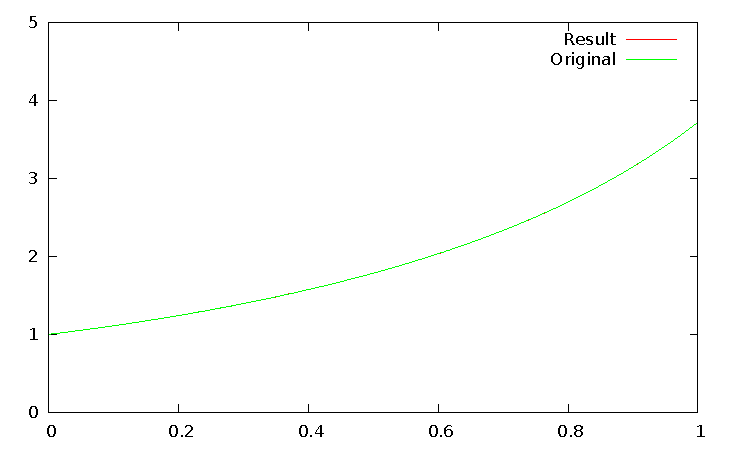
\includegraphics{../plots/btest1.pdf}

\subsubsection*{Тест 2}

Дана следующая краевая задача на отрезке $[0, 1]$:
$$
y'' + y' - 2y = 0,
$$

$$
\begin{cases}
  y(0) + y'(0) = 1, \\
  y(1) = 0
\end{cases}
$$

Аналитическое решение задачи:
$$
y = -\frac{e^{3 - 2x} - e^x}{2 + e^3}
$$

Результат работы программы, максимальная ошибка составила $5.91875 \cdot 10^{-5}$:

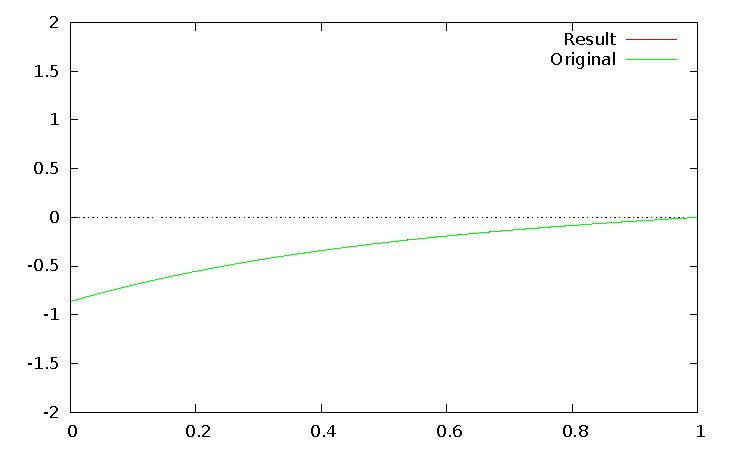
\includegraphics{../plots/btest2.pdf}

\subsubsection*{Тест 3}

Дана следующая краевая задача на отрезке $[0, 1]$:
$$
y'' = \sin x
$$

$$
\begin{cases}
 y'(0) = 1,
 y(1) = 1
\end{cases}
$$

Аналитическое решение задачи:
$$
y = 2x - \sin x - 1 + \sin 1
$$

Результат работы программы, максимальная ошибка составила $1.53456 \cdot 10^{-7}$:

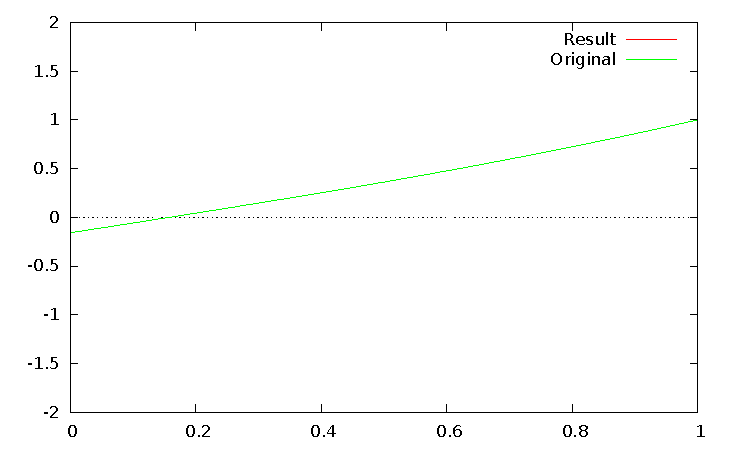
\includegraphics{../plots/btest3.pdf}

\subsubsection*{Тест 4 (предложенный вариант)}

Дана следующая краевая задача на отрезке $[0.5, 0.8]$:
$$
y'' + 2 x^2 y' + y = x,
$$

$$
\begin{cases}
 2 y(0.5) - y'(0.5) = 1, \\
 y(0.8) = 3
\end{cases}
$$

Аналитическое решение получить не удалось.

Результат работы программы:

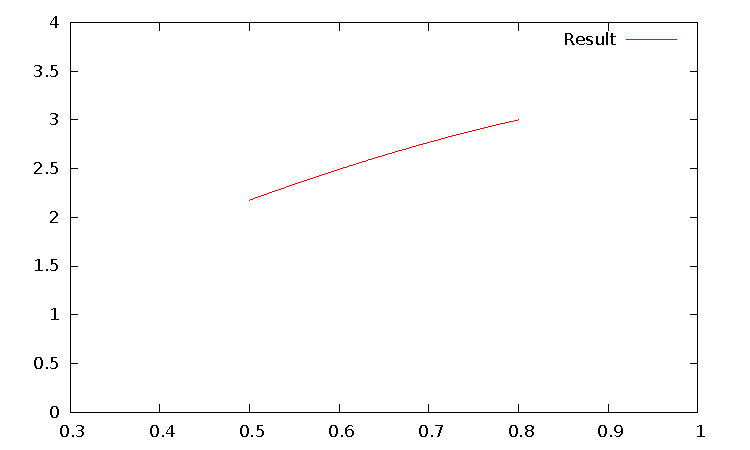
\includegraphics{../plots/btest4.pdf}

\subsection*{Исходный код}
\lstinputlisting[caption={Функция решения краевой задачи}]{../boundary.c}
\lstinputlisting[caption={boundary.h}]{../include/boundary.h}

\newpage

\section*{Выводы}

Численные методы решения дифференциальных уравнений и систем дифференциальных уравнений позволяют с достаточно высокой точностью
получать решения уравнений в условиях, когда получить аналитическое решение не представляется возможным.

Методы не очень сложны для вычислений, рассмотренные выше имеют алгоритмическую сложность $O(n)$, что позволяет проводить требуемые
вычисления практически на любых вычислителях с приемлемой скоростью.

При необходимости увеличения точности вычисления, как правило, достаточно уменьшить длину отрезка сеточной функции, что приведёт
к увеличению времени работы.

Способ решения с использованием сеточных функций позволяет также применять данные методы к дискретным функциям (например, значениям,
полученным с сенсоров или датчиков).

\newpage

\section*{Приложение 1. Исходный код проекта}

Исходные коды проекта доступны на Github: https://github.com/webconn/cmc\_DiffEquations

Ниже приведены исходные коды модулей, не описанные выше.

\lstinputlisting[caption={Исходный код интерфейса программы (файл main.c)}]{../main.c}
\lstinputlisting[caption={Библиотека для работы с сеточными фунциям (файл grid.c)}]{../grid.c}
\lstinputlisting[caption={grid.h}]{../include/grid.h}
\lstinputlisting[caption={Тестирующие функции для решателей (файл test.c)}]{../test.c}
\lstinputlisting[caption={test.h}]{../include/test.h}
\lstinputlisting[caption={Описание дифференциальных уравнений первого порядка из тестов (файл func1.c)}]{../func1.c}
\lstinputlisting[caption={Описание систем ДУ первого порядка (файл system1.c)}]{../system1.c}
\lstinputlisting[caption={Описание дифференциальных уравнений второго порядка из тестов (файл func2.c)}]{../func2.c}

\end{document}          